%----------------------------------------------------------------------------
\chapter{Háttérismeretek}
\label{chp:background}
%----------------------------------------------------------------------------
Ebben a fejezetben a feladat megértéséhez szükséges technológiákat mutatom be röviden.

%----------------------------------------------------------------------------
\section{Virtuális gépek}
%----------------------------------------------------------------------------
\begin{itemize}
  \item általában egy virtuális gép mire jó
  \item	vagrant szerepe virtuális gépek létrehozásában/konfigurálásában
\end{itemize}

Érdemes pár szót ejteni a virtuális gépekről, hiszen ezek terítése a programunk célja. Virtuális gépet használva egy számítógépes környezetet szimulálhatunk, ezen belül is \ldots platform virt \ldots Virtuális   

%----------------------------------------------------------------------------
\section{Peer-to-peer fájlátvitel} 
\label{sect:p2p}
%----------------------------------------------------------------------------
A Peer-to-Peer(P2P) hálózat olyan, aminek a csomópontjai nem egy kitüntetett géppel 
kommunikálnak, hanem közvetlenül egymással. A klasszikus kliens-szerver és a P2P hálózat felépítését
a~\ref{fig:networkcomparison}~ábra szemlélteti.

\begin{figure}[ht]
	\centering
	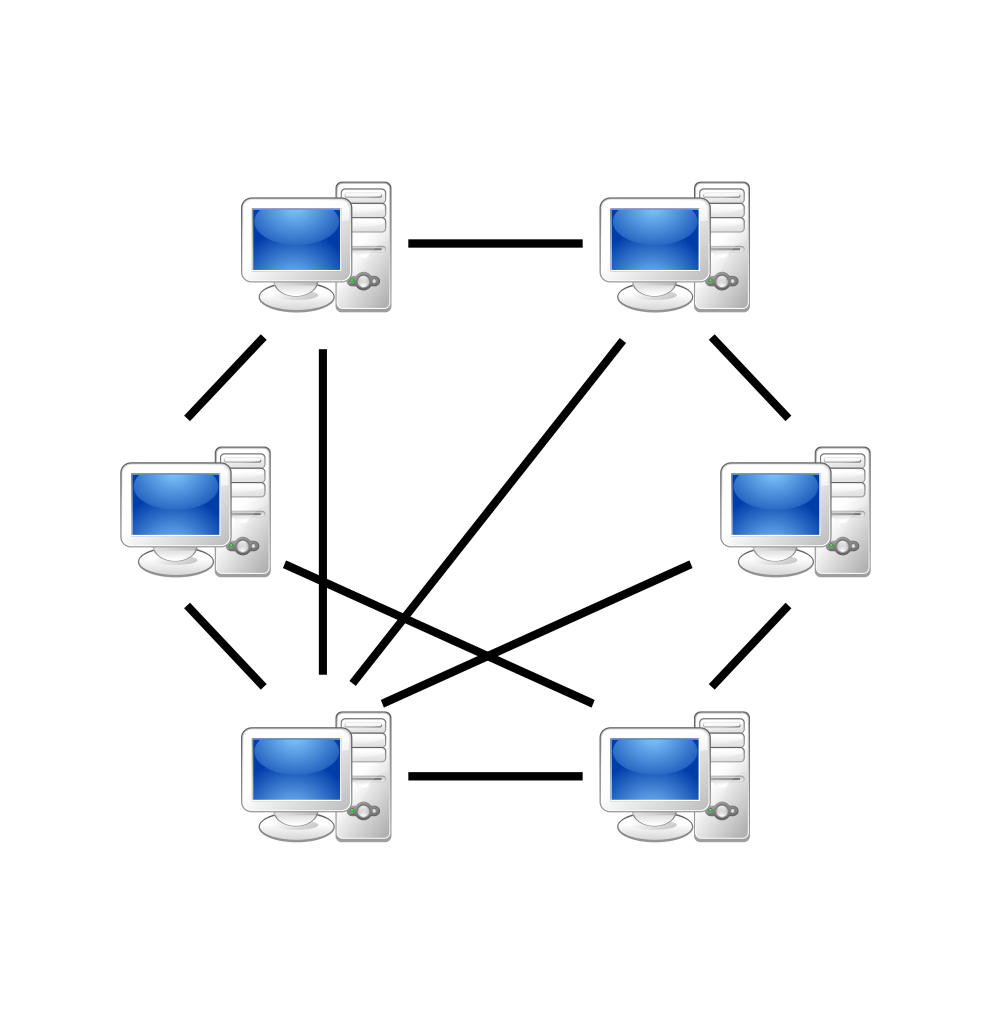
\includegraphics[width=50mm, keepaspectratio]{figures/P2P-network.png}\hspace{1cm}
	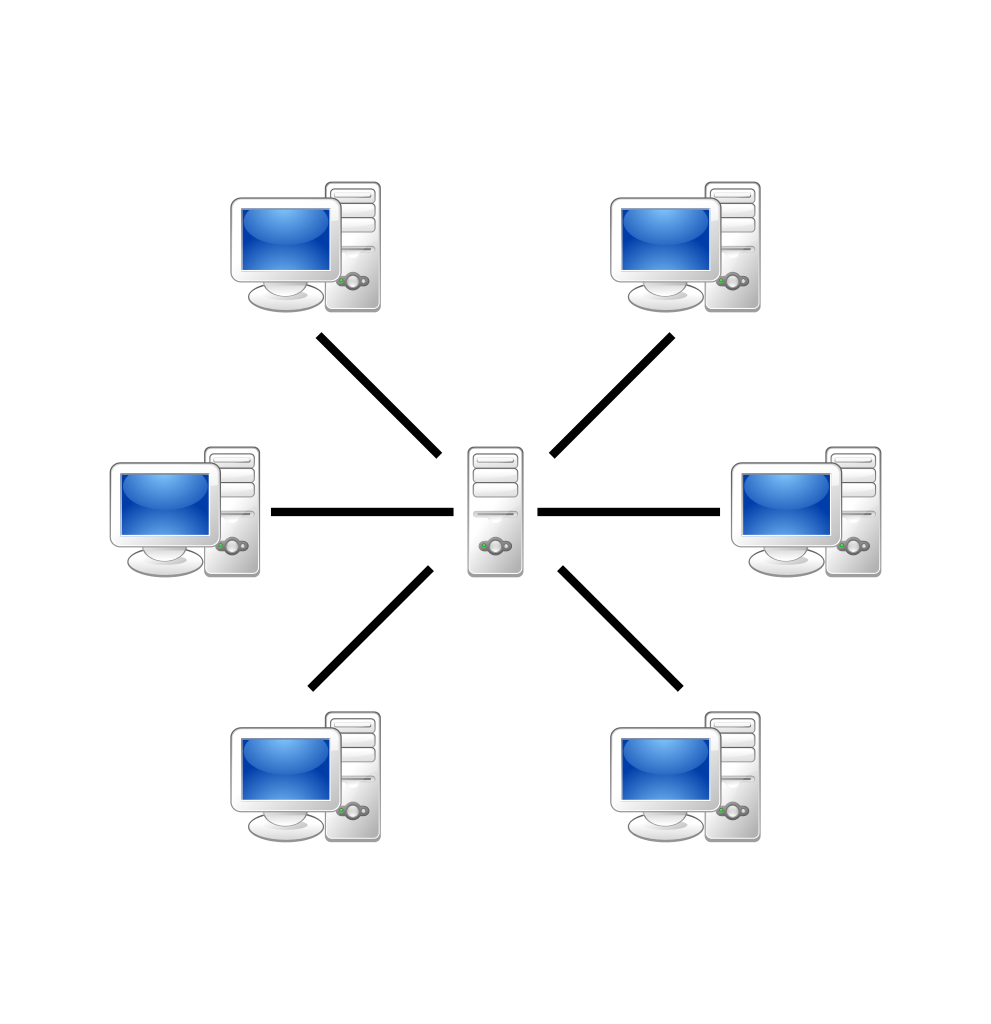
\includegraphics[width=50mm, keepaspectratio]{figures/Server-based-network.png}
	\caption{P2P és kliens-szerver alapú hálózat.}%TODO forrásmegjelölés
	\label{fig:networkcomparison}
\end{figure}

P2P hálózat használatának fő előnye a robusztusság és a skálázhatóság, mivel nincs központi elem,
aminek a meghibásodása szolgáltatáskiesést okozhatna, illetve a hálózat min (például P2P alapú fájlmegosztás esetén a letöltés mellett fel is tölt). Hátrányai közül a két legjelentősebb a nehezebb karbantarthatóság, és az internetszolgáltató-oldali forgalomkorlátozások miatt fellépő sebességproblémák.\\
A P2P alapú technológiák egyik legnagyobb felhasználási területe a tartalomszolgáltatás, ezen belül
az egyik legismertebb ilyen technológiát használó protokoll a Bittorrent. A Bittorrent~\cite{cohen2008bittorrent} protokollt
fájlmegosztásra használjuk, a mögötte álló alapvető ötlet az, hogy a megosztandó fájlokat
feldaraboljuk, és a letöltőknek ezeket a darabokat nem ugyanolyan sorrendben adjuk oda, így ők a
hiányzó darabokat egymástól is tudják tölteni. Ahhoz, hogy a letöltők megtalálják egymást, illetve a kész fájlt feltöltőket az ún. tracker segít, ami adott átvitel résztvevőinek (a ``swarm'') adatainak tárolásáért felel. A Bittorrent terminológiájában a teljes fájlal rendelkező, már csak feltöltést végzőket seed-nek, a letöltőket, akik persze fel is töltenek leecher-nek vagy peer-nek nevezik. A tracker kiesése esetén léteznek más módszerek is a többi swarm-tag megtalálására, többek között a DHT\cite{rescorla2006introduction}(distributed hash table - elosztott hashtábla) használata, viszont esetünkben ez nem opció, mert az egyetem szabályzata tiltja a Bittorrent protokoll használatát (legalábbis a ``nagyvilág'' felé), a DHT bekapcsolása esetén pedig nem tudjuk a laborgépeinken futó torrentkliensek közti forgalmat a helyi hálóra izolálni.\\
Látszik, hogy torrent-alapú fájlátvitel megvalósításához minimum mikre lesz szükségünk:
\begin{itemize}
	\item Minden laborgépen egy torrentkliensre
	\item Saját torrent tracker-re
	\item Egy olyan programra, ami ezek működését vezérli
\end{itemize}
Gépeinkre telepítendő torrentkliens esetében az rtorrent-re\cite{sundell2012libtorrent} esett a választás, mivel szükségünk van arra, hogy olyan klienst használjunk, amit a háttérben is tudunk futtatni, illetve az állapota valami módon távolról is lekérhető legyen. Az rtorrent rendelkezik egy XMLRPC\cite{merrick2006xml} alapú interfésszel, aminek segítségével távolról is vezérelhetővé válik. Ilyen interfészt használ a számos rtorrent-hez írt webes felület is, például a legismertebb ruTorrent\cite{rutorrent}. Természetesen minden rtorrent-et futtató gépre telepítenünk kell egy webszervert is, ami az XMLRPC kéréseinket eljuttatja magának a torrentkliensnek, itt a választás az apache-ra\cite{fielding1997apache} esett főleg könnyű telepítése és konfigurálása miatt.\\
Tracker-ből az opentracker nevű került fel egy gépre (az egyszerűség kedvéért arra, amelyiket a terítések során seed-nek fogunk használni), választásunk rá azért esett, mert különösebb funkcionális különbség nincs a lehetséges jelöltek között, ezt viszont könnyen lehet telepíteni a laborgépeken futó operációs rendszer csomagkezelőjéből. Amiről még eddig nem esett szó, az a protokoll működéséhez szükséges, metaadatokat tartalmazó fájl, a torrentfájl. Ez tárolja az adott letöltéshez tartozó fájlok hash-eit, amik adott fájl tartalmából előállított egyedi hexadecimális számok, tulajdonságuk, hogy ugyanarra a fájlra mindig ugyanaz a szám áll elő, másikra pedig (szinte) biztosan különböző, ezek alapján tudjuk ellenőrizni a letöltött adatok hibamentességét. A torrent fájl tartalmazza még ezen kívül a küldendő fájlok mappastruktúráját, metaadatait (pl. fájlnév, fájlméret) és a tracker címét. A torrentkliens és a tracker egy torrentfájlra az infohash alapján hivatkozik, ami a torrentfájl hash-ének kódolásával kapható meg, erre nekünk később akkor éesz szükségünk, amikor majd a terítés közben annak állapotának lekérésekor hivatkozni akarunk egy átvitelre.\\
Torrentfájlok létrehozására az mktorrent-et\cite{mktorrent} fogjuk használni.


%----------------------------------------------------------------------------
\section{Metamodellezés}
%----------------------------------------------------------------------------
\begin{itemize}
  \item modellezés mire jó
  \item	használata hogyan segíthet a feladat megoldásában
  \item eclipse EMF-et használva ez hogyan teljesül
\end{itemize}